In this chapter we will describe: 
\begin{itemize}
	\item The steering behaviors we implemented.
	\item How we implemented these steering behaviors.
	\item The issues and problems we faced while implementing the steering behaviors and how we solved these issues.
	\item How steering behaviors can be combined within our game.
\end{itemize}
A class diagram about all of the classes that are relevant to the steering behaviors can be found at the bottom of this chapter.
\subsection{Behaviors}
We implemented the following steering behaviors: 
\begin{itemize}
	\item Seek. \\ 
	Will steer the agent towards a target within the game.
	\item Flee. \\
	Will steer the agent away from a target within the game.
	\item Arrive. \\
	Will steer the agent towards a target within the game and will decelerate as the agent gets closer to the target position.
	\item Follow Path. \\ 
	Will steer the agent along a path. 
	Uses seek to reach all the waypoints but the last waypoint within the path. 
	Arrive is used for the last waypoint.
	\item Pursuit. \\
	Will steer the agent towards a target agent.
	\item Evade. \\ 
	Will steer the agent away from a target agent.
	\item Offset Pursuit. \\
	Will steer the agent towards a target agent while keeping a distance between them.
	\item Explore. \\
	Will make the agent explore a queue of Powerups.
\end{itemize}
Our implementation supports the following summing methods: 
\begin{itemize}
	\item Weighted truncated sum.
	\item Prioritization.
	\item Prioritized dithering.
\end{itemize}
\subsection{Issues and Solutions}
We mainly just rewrote the source from the Programming Game AI by Example book by Mat Buckland into C\# so we didn't have too many problems. We had some issues with updating the Velocity/Heading of the agent's and calculating the steering force based on the elapsed time. The measurement of elapsed time that Mat Buckland uses didn't seem to be documented within the source so it took some adjustments to get it about right. \\\\ We used a different implementation for the Offset Pursuit than the book did. The reason for this is that this seemed like a simpler implementation with the same effect.

\begin{figure}[H]
	\centering
	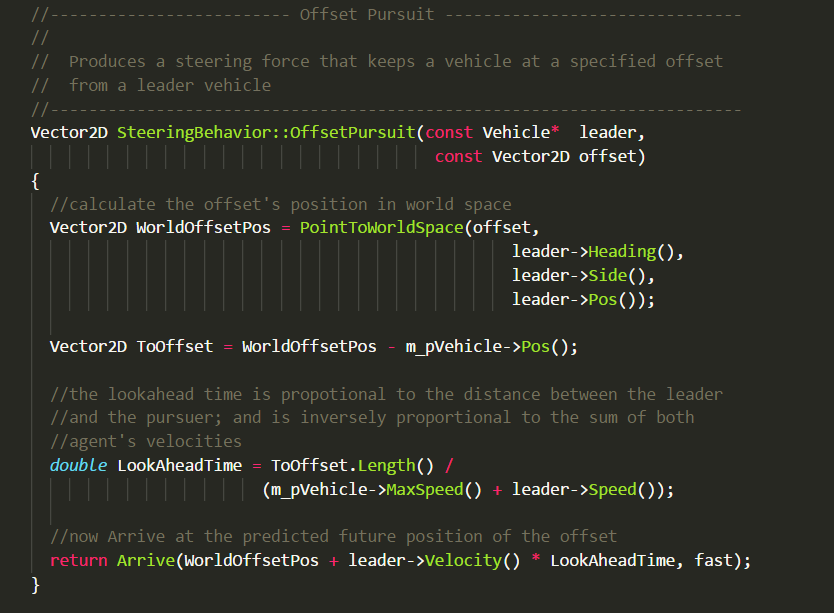
\includegraphics[width=0.7\linewidth]{Images/offsetsource}
	\caption{Original Offset Pursuit.}
	\label{fig:offsetimplementation}
\end{figure} 
\begin{figure}[H]
	\centering
	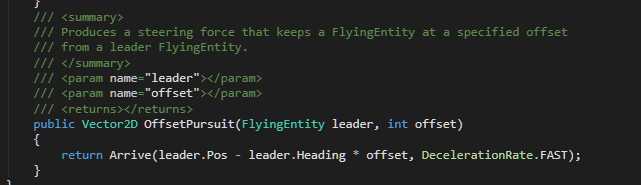
\includegraphics[width=0.7\linewidth]{Images/offsetimplementation}
	\caption{Implementation of Offset Pursuit.}
	\label{fig:offsetsource}
\end{figure} 
We also had some issues with oscillation which were solved by creating a threshold.
We basically made it so that if the agent is within a certain very close distance to the target position the agent's position will be transformed into the target position after finding an article about the issue. \cite{steeringissue}. 
\subsection{Combining Steering Behaviors}
Combining multiple steering behaviors is very easy since we use a bit operator system for it (just like the book did). 
\begin{figure}[H]
	\centering
	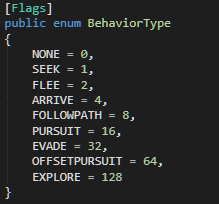
\includegraphics[width=0.7\linewidth]{Images/bitoperatorsflagenum}
	\caption{Behaviour flags.}
	\label{fig:behaviourflags}
\end{figure} 
\begin{figure}[H]
	\centering
	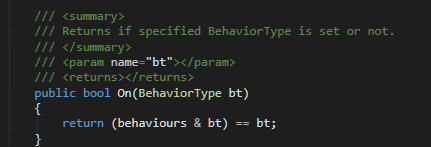
\includegraphics[width=0.7\linewidth]{Images/bitoperatorson}
	\caption{Method for asserting if a behavior is enabled or not.}
	\label{fig:offsetsource}
\end{figure} 
\begin{figure}[H]
	\centering
	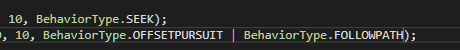
\includegraphics[width=0.7\linewidth]{Images/multiplebehaviors}
	\caption{Combining steering behaviors.}
	\label{fig:multiplebehaviors}
\end{figure}

\subsection{Class Diagram}
\begin{figure}[H]
	\centering
	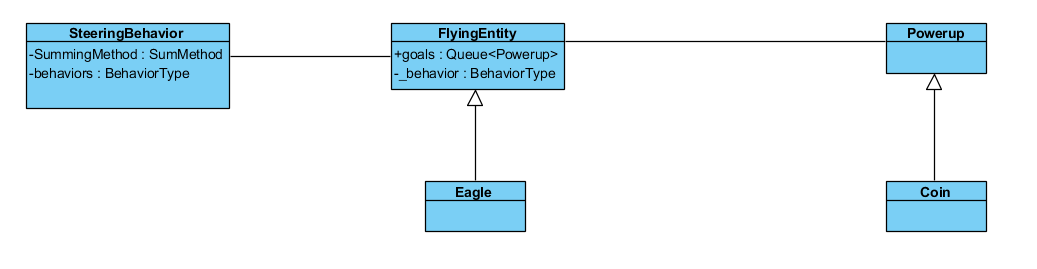
\includegraphics[width=0.7\linewidth]{Images/steeringclassdiagram}
	\caption{Class diagram of classes that are relevant to steering.}
	\label{fig:steeringclassdiagram}
\end{figure}